

\section{Questão 6}



\subsubsection{Identifique uma sequência de tramas que corresponda a um processo de associação completo entre a STA e o AP, incluindo a fase de autenticação.}

    \par Um processo de associação completo envolve vários tipos de tramas como: \textit{Association Request}, \textit{Association Response}, \textit{Authentication} e, por fim, \textit{Acknowledgement}. Assim, desenvolvemos um filtro que pesquisasse todas estas tramas para facilitar a pesquisa de todo o processo. Os valores dos subtipos no filtro foram utilizados de acordo com o anexo fornecido dos docentes. Apresentamos, então, o filtro desenvolvido seguido do processo de associação identificado:
    
    \vspace{10pt}
    \begin{minipage}{\linewidth}
        \centering
        \fbox{
        \parbox{250pt}{
		    (wlan.fc.type\_subtype $==$ 0x00) \textbf{or} (wlan.fc.type\_subtype $==$ 0x01)
		    \textbf{or} (wlan.fc.type\_subtype $==$ 0x0b) \textbf{or} (wlan.fc.type\_subtype  \hspace{22pt}$==$\hspace{22pt} 0x1d) 
        }
    }
    \end{minipage}

    \begin{figure}[H]
        \centering
        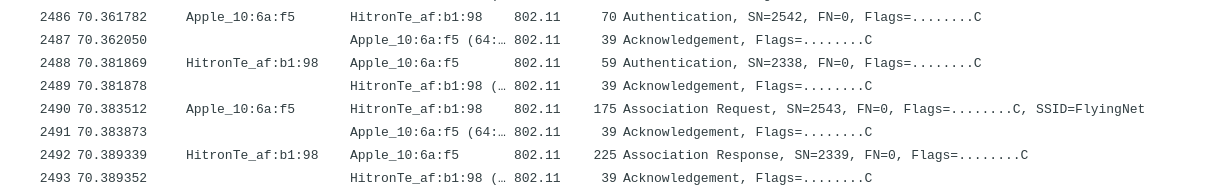
\includegraphics[width=500pt]{Prints/Questao6/rc1.png}
        \caption{Processo de associação completo entre a STA e o AP} \label{questao6-1}
    \end{figure}








\subsubsection{Efetue um diagrama que ilustre a sequência de todas as tramas trocadas no processo.}

    \par A partir das tramas obtidas na alínea anterior, desenvolvemos o seguinte diagrama ilustrando as mensagens trocadas entre STA e o AP durante o processo de associação:

    \begin{figure}[H]
        \centering
        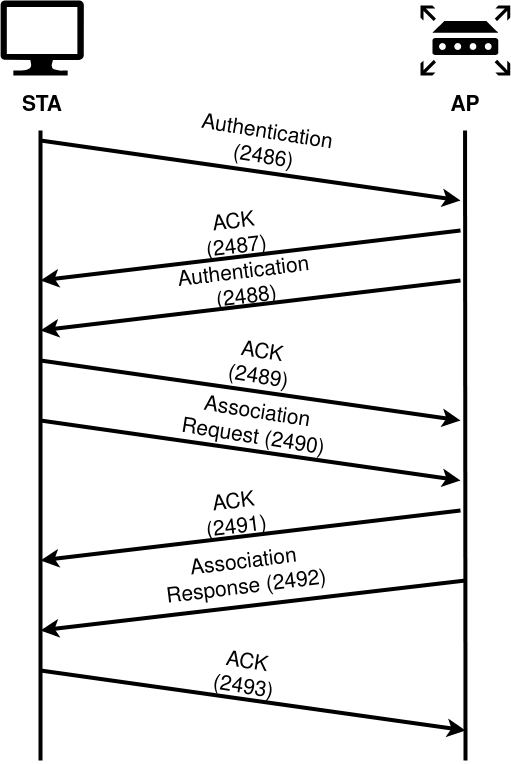
\includegraphics[width=150pt]{Prints/Questao6/STA-AP.png}
        \caption{Sequência de tramas trocadas durante o processo} \label{questao6-2}
    \end{figure}